\section{Проблематика выбора объектов}
\begin{frame}{C чем мы имеем дело?}
	%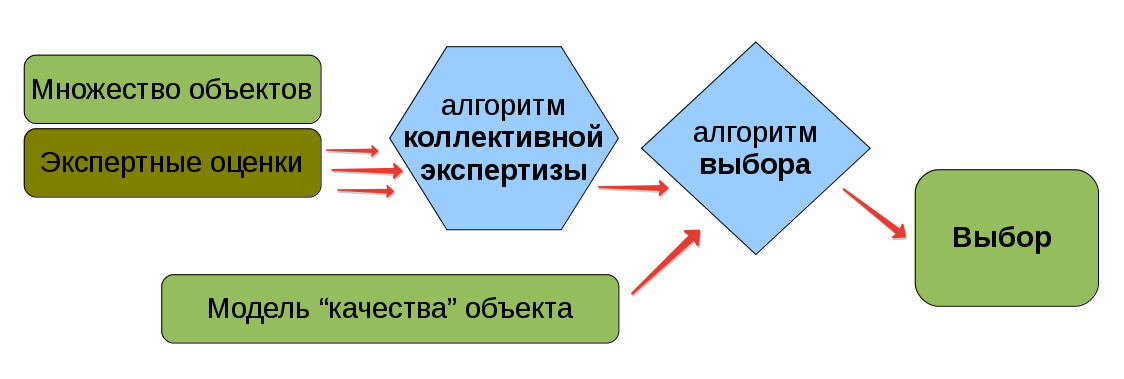
\includegraphics[width=0.8\linewidth]{./pic/globalscheme}
 	\begin{columns}
 		\column{0.50\textwidth}
 			Есть $n$ объектов, у каждого объекта % составителем методологии выбрано
 			есть $m$ параметров. Модель: {\small {\em независимые} нечёткие элементы} 
			\\ \vspace*{2mm}   % характеризуем с совсем разных сторон
 			$\tilde x_{ij} \in X$, {\footnotesize $i = 1 \ldots n$, $j = 1 \ldots m$} 
 			\\ \vspace*{3mm}
 			$x_{ij} \in X$ -- их значения (неизвестны), где $X$ --  числовое множество.
 			\\[1.1ex] {\small Например, $X = \{1, \ldots, 10\}$ --  множество баллов по десятибалльной шкале} 
 			%некое выпуклое подмножество действительной оси
 		\column{0.50\textwidth}
 			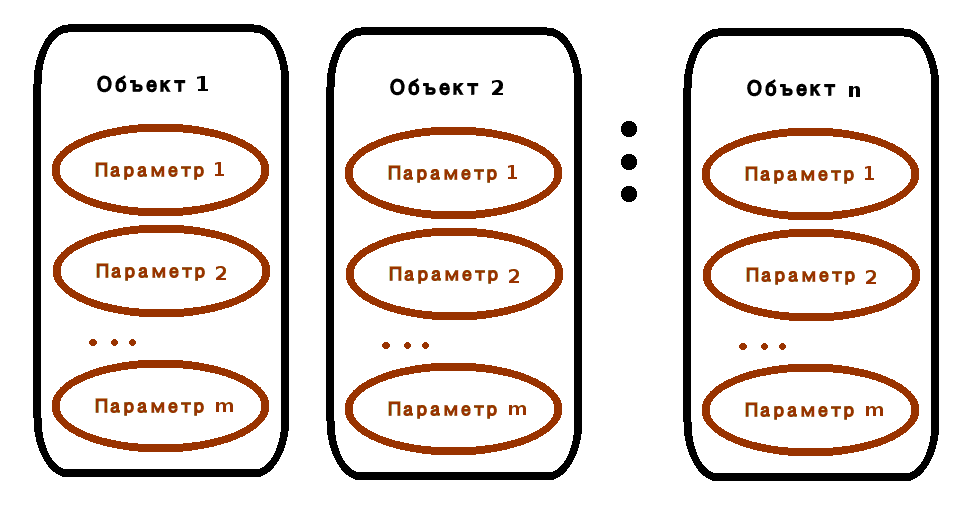
\includegraphics[width=1.0\linewidth]{./pic/theobjects}
 	\end{columns}
 	
	\vspace*{5mm}
	\begin{columns}
		\column{0.60\textwidth}
		Экспертные оценки -- это распределения $\tilde x_{ij}$: 
		{\large \begin{center} \hspace{-8mm}  $\p_{ij}^{(r)}( \cdot )$ \end{center} }
		{\footnotesize где $i = 1 \ldots n$ -- номер объекта, $j = 1 \ldots m$, -- номер параметра, $r = 1 \ldots R$ -- номер эксперта}.  
		\column{0.40\textwidth}
		\begin{center}
			\vspace*{-6mm}
			%   {\small Примеры оценок:}
			  {\scriptsize {Примеры оценок: значения $\p(x)$ показаны цветом, $x \in \setTen$}}
			  \\ \vspace*{2mm}
			  \resizebox{1.0\linewidth}{!}{\showevDisplayFullScale{./pic/chapter01-tech01.dat}}
		\end{center}
	\end{columns}

 \end{frame} %===========================

\begin{frame}{Процесс выбора объектов}
	 
	 \vspace*{-3ex}
	 \hspace{2mm} Модель <<качества>>  объекта:
	  \\[1ex] \hspace{25mm} { \small \tikz { \node  (n1) { \light{монотонна и задана заказчиком экспертизы}  }; } }
	 \\  \hspace{5mm}  $x_i = \tikz[baseline] { \node[anchor=base, fill=\mygreen] (t1) {$f$}; } (x_{i1}, ..., x_{im}),\; x_i \in X$ -- <<качество>> объекта с номером $i$; 
	 \\  \hspace{5mm} например, для $x_{i1}, x_{i2}$ можно взять $\displaystyle f(x_{i1}, x_{i2}) = \frac{1}{2} (x_{i1} + x_{i2})$. 
	\begin{tikzpicture}[overlay]
		\path[->] (n1.west) edge  (t1.north east);
	\end{tikzpicture}
	\vspace*{1ex}
	\begin{center}
	      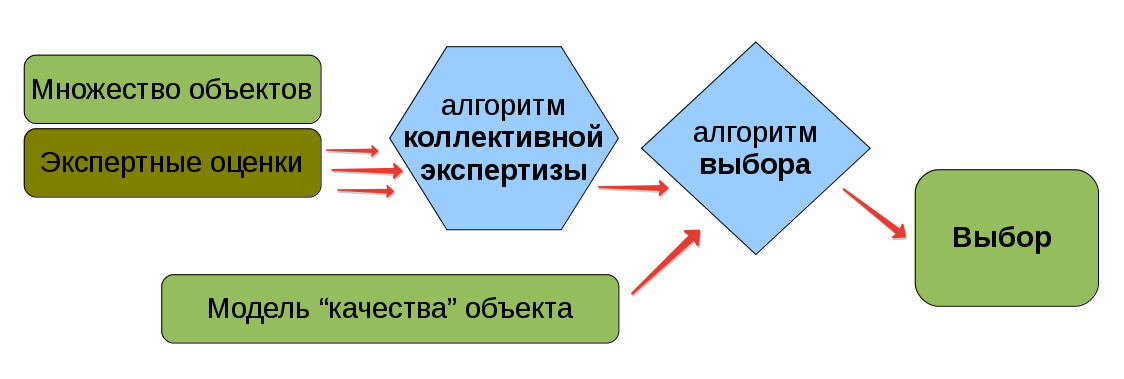
\includegraphics[width=0.9\linewidth]{./pic/globalscheme}
	\end{center}      
 \end{frame} %===========================
 
\section{Задача и алгоритм выбора}
\begin{frame}{Задача выбора объектов}
	
	{ Пусть $t = (x_{11}, ..., x_{nm}) \in T = X^{nm}$ -- вектор значений параметров всех объектов}.	
	 {\small Например, в случае $X = \{1, \ldots, 10\}$ размер пространства $\abs{T} = 10^{nm}$}. 
	\\[1.5ex] Пусть $d \subset \setN$ -- какой-то выбор; $\delta_t$ -- {\em верный} выбор {\small при известном $t$}. %нсли бы знали x_i
	\begin{gather*}
	      \abs{d} = \abs{\delta_t} = k \text{ -- задано; } \delta_{t} \define= \{i_1, \mydots, i_k\}: \forall\, i \in \delta_t,\; \forall\, i' \in \setN \setminus \delta_t: \\ f(x_{i1}, ..., x_{im}) > f(x_{i'1}, ..., x_{i'm}).
	 \end{gather*}
	%\vspace*{-2mm}
	\vspace{-4ex}
	\begin{center}
	 Работает \emph{один} эксперт {\small (или используется результат коллективной экспертизы)}.
	 
	Оценки $\p_{ij}$ %,{\footnotesize $i = 1 \ldots n$, $j = 1 \ldots m$},
	    порождают возможность $\P(\{t\}) = \p(t)$ через их совместное распределение $\p(x_{11}, \ldots, x_{nm}) = \inf_{i, j}\,\p_{ij}(x_{ij})$, {\footnotesize $i = 1 \ldots n$, $j = 1 \ldots m$}.
	    
	%\end{center}
	% каждый эксперт оценивает все параметры, которые являются разложением макропараметров качества объектов.
	% в данной задаче всюду используется одна и та же шкала возможности
	%\\ \vspace*{2mm} $\P(\{t\}) = \p(t)$.
	%\vspace*{-2mm}
	%\begin{center}
	%      \vspace*{-1mm}
	     \textbf{Задача }{\small (ставится впервые)}: \tikz[baseline] {  \node[anchor=base, fill=\mygreen]{ $\P(\Eps(d)) \sim \underset{d} \min$ }; },
	     где $\Eps(d) = \{d \neq \delta_t\}$. % размер подможества.
	     \\[1ex] {\footnotesize Оптимальное решение может быть не единственным!}
	\end{center}
\end{frame} %===========================

\begin{frame}{Алгоритм выбора: работа с  возможностью}
\vspace*{-4mm} 
\begin{gather*}
%	\text{\small Возьмем любое событие $A$, в частности, $A= \Eps(d)$.}
	%\hspace*{4mm} 
	\mathsmaller{  t = (x_{11}, \ldots, x_{nm})  \in T = X^{nm}, x_{ij} \text{ -- его коордианты}, {i = 1 \ldots n, j = 1 \ldots m}.}
	\\[2ex] \P(A) = \text{?..  перебрать все $t \in T$ можно за $O(\abs{X}^{nm})$ операций}.
	\\ \P(A) > p_0 \in \zo \text{?.. Решается за $O(nm)$ из-за свойств $\sup$ и $\inf$.}
	%\\[5pt]  \hspace*{4mm} {\small  t = (x_{11}, \ldots, x_{nm})  \in T = X^{nm} \text{ -- вектор значений параметров всех объектов} }
\end{gather*}
{\large 
  \hspace{6mm} $\P($\tikz[baseline]{\node[anchor=base, fill=\mygreen](nPA){$A$};}$\displaystyle  ) = \sup_{ t \in A}\;\inf_{i, j}\,\p_{ij}(x_{ij})\; $
  \hspace{8mm} \tikz[baseline]{\node[anchor=base, fill=\mygreen](nB){$B$};}$ \define= \{t:  \forall i,j\; \p_{ij}(x_{ij}) > p_0\}$
}
\begin{center}
    \tikz{ \node (tSets) { 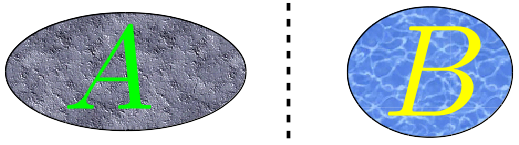
\includegraphics[width=0.5\linewidth]{./pic/algo_sets_simple} };}
    
   % {\small Для нахождения $\P(A)$ перебор всех векторов $t$ потребовал бы $O(\abs{X}^{nm})$ операций!}
    Разработан алгоритм, который за время $O(nm)$ позволяет проверить, пересекаются ли $\Eps(d)$ и $B$. Если и только если пересекаются, $\P(\Eps(d)) > p_0$.
\end{center}
\begin{tikzpicture}[overlay]
	\path[->] (nPA.south) edge [bend right] (tSets.west);
	\path[->] (nB.south) edge (tSets.north north east);
\end{tikzpicture}
\end{frame} %===========================

% == eof == eof ===